%% ==============================================================================
%%
%%  Document settings and macro definitions
%%
%% ==============================================================================

\documentclass[a4paper,10pt,bibtotoc]{scrartcl}
\usepackage{a4wide,usg}

%% Do NOT remove: required to extract SVN information
\svnInfo $Id$

%% Adjust page footer
\fancyfoot[LE,LO]{LOFAR-USG-ICD-00DRAFT: TBB Subband Data}
\fancyfoot[RE,RO]{\textsc{lofar} Project}

%% Additional typesetting macros

\newcommand\sumline[2]{%
  \hbox to \linewidth{%
    \strut
    \parbox[t]{.85\linewidth}{\strut #1\strut}\hss
    \parbox[t]{.15\linewidth}{\raggedleft\strut #2\strut}%
  }
}

\newcommand\kw[0]{$KW$}

%% ==============================================================================
%%
%%  Document
%%
%% ==============================================================================

\begin{document}

\title{Draft for LOFAR Data Format ICD \\ TBB Subband Data \\
  {\normalsize Document ID: LOFAR-USG-ICD-00DRAFT} \\ 
  {\normalsize Version 0.02.01} \\
  {\normalsize SVN Repository Revision: \svnInfoRevision}}
\author{M.~Eikelboom}
\date{\small{SVN Date: \svnInfoDate}}

\maketitle

\tableofcontents

\clearpage

%%_______________________________________________________________________________
%% Change record of the document

\section*{Change record}
\addcontentsline{toc}{section}{Change record}

\begin{center}
  %% Table head
  \tablefirsthead{
    \hline
    \sc Version & \sc Date & \sc Sections & \sc Description of changes \\
    \hline
  }
  \tablehead{
    \multicolumn{4}{r}{\small\sl continued from previous page} \\
    \hline
    \sc Version & \sc Date & \sc Sections & \sc Description of changes \\
    \hline
  }
  %% Table tail
  \tabletail{
    \hline
    \multicolumn{4}{r}{\small\sl continued on next page} \\
  }
  \tablelasttail{\hline}
  %% Table contents
  \begin{supertabular}{lllp{10cm}}
    0.01.00 & 2011-06-22 & all & First version of draft submitted. \\
    0.02.00 & 2011-06-23 & all & Matching up layout with other ICDs. \\
    0.02.01 & 2011-07-06 & all & Matching up group type attributes and
    notation; consolidation of labels to refer to standard sections
    and tables. \\
 \end{supertabular}
\end{center}

\input version_numbering

\input notation

\section*{Acknowledgements}

t.b.a.

\clearpage

%%_______________________________________________________________________________
%%                                                                   Introduction

\section{Introduction}
\label{sec:introduction}

\subsection{Purpose and scope}
\label{sec:purpose and scope}

This document is an attempt to set up a draft version to describe the internal structure
of and the interface to the LOFAR subband data. It is modelled after
document \cite{lofar.icd.001} which describes the Data Format for time
series. Subband data -- i.e. the frequency bands of resampled voltage
output, as received by the individual LOFAR dipoles -- represent an
alternative to the primary input data to the UHECR (Ultra-High-Energy
Cosmic Rays) analysis pipeline(s) and have to be considered as a basic
form in which the received radio signals are present within the LOFAR system.

\subsection{Context and motivation}
\label{sec:context and motivation}

The fundamental difference between analysis for LOFAR Cosmic Ray (CR)
data with respect to other LOFAR Key Science Projects (KSP) is the
fact that processing starts from the raw digitized time-series data
delivered by the individual dipoles of the LOFAR telescope. For the
subband mode of the TBB's, these time series are resampled by DFT.
This approach is required to provide the necessary time-resolution --
essentially down to the time-interval at which the analog signal is
sampled -- to detect, identify and investigate the radio pulses from
Extensive Air-Showers (EAS) originating form high-enery cosmic rays. 

Based on a number of considerations we have chosen the HDF5 data
format as common wrapper for the standard LOFAR data products (or at
least a considerable fraction thereof). The goal is to create along
with the definitions of the standard data product also an
infrastructure which will enable LOFAR users to access and manipulate
such data -- this document therefore also serves as reference for the
implementation with the Data Access Library (DAL). 

\input applicable_documents

%% ______________________________________________________________________________
%%                                                              Section: Overview

\section{Overview}
\label{sec:overview}

This document is structured as follows: Section \ref{sec:structure}
will describe fundamental overall structure, including a statement of
the primary data product format, HDF5. These conventions will also
include names, meaning, and physical units that may be used to
generate and interpret the data files. Section \ref{sec:detailed structure} 
will present a detailed specification for the data, including a
description of the structure of a LOFAR TBB data naming
conventions, units, physical quantities. Section 5 will provide a
detailed description of the group and dataset structures contained
within the LOFAR TBB Subband file format, as well as meta-data in
the form of HDF5 dataset headers.

%%_______________________________________________________________________________
%%                                              Section: Organization of the data

\section{Organization of the data}
\label{sec:structure}

\subsection{High level LOFAR TBB Subband file structure}

A LOFAR  TBB Subband data file will adhere to the following guidelines:\\

A LOFAR TBB Subband data file will be defined within the context
of the HDF5 file format.  A LOFAR TBB Subband HDF5 file structure
will comprise a primary group, a "root group" in HDF5 nomenclature,
which may be considered equivalent to a primary header/data unit (HDU)
of a standard multi-extension FITS file.  This primary group will
consist only of header  keywords (“attributes” in HDF5 nomenclature)
describing general properties of an observation, along with pointers
to contained subgroups.  These subgroups will comprise an arbitray
number of ``StationGroups'' (\textit{§ 4.2}), where a Station Group
will contain data and meta-data produced by an individual LOFAR
station. 

The figure below shows the basic organization of the dataset within
the HDF5 format. The hierarchical structure essentially follows the
hierarchical structure of LOFAR itself, i.e. in a top-down approach
from array through stations down to individual dipoles. The grouping
of multiple antennas/dipoles into a station is mirrored by the
collection of dipole datasets into a station group.

\subsection{Overview of TBB Groups}

\begin{comment}
Expand the descriptions of the groups - don't just put in references?
\end{comment}

\begin{enumerate}
\item \textbf{Root group}. The root level of the file contains the
  majority of associated meta-data, describing the circumstances of
  the observation. These data attributes include observation time
  (start and end), frequency window (high band vs. low band, filters)
  and other important characteristics of the dataset. See
  section \ref{sec:root group} for further details.
\item \textbf{System Logs Group} (\verb|SYS_LOG|). This is a catch-all
  envelop encapsulating information about all the system-wide steps of
  processing which are relevant to the entire observation, such as
  parameter sets and processing logs. See Sec.~\ref{sec:sylog group} for details.
\item \textbf{Station group} See section \ref{sec:station group} for
  further details.
\item \textbf{Station calibration group}. See
  section \ref{sec:station calibration group} for further details.
\item \textbf{Station trigger group}. See section \ref{sec:station
    trigger group} for further details.
\item \textbf{Dipole group}
\item \textbf{Dipole calibration group}
\item \textbf{Dipole dataset}
\end{enumerate}

%%_______________________________________________________________________________
%%                                                    Detailed Data Specification


\subsection{Hierarchical structure}
\label{sec:hierarchical structure}

\begin{figure}[htb]
  \centering
  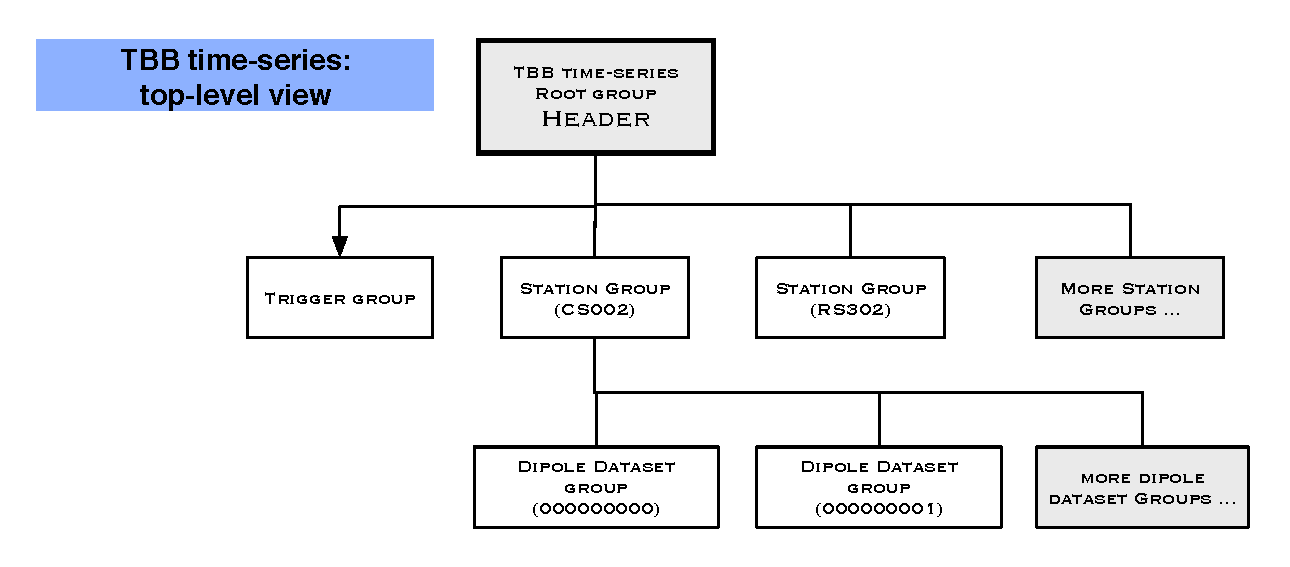
\includegraphics[width=\textwidth]{figures/TBB_highlevel_new.eps}
  \caption{Hierarchical structure of a TBB subband dataset; the
    internal organization of the data follows the hierarchical
    organization of the LOFAR system.}
  \label{fig:TBB_highlevel}
\end{figure}

\begin{lstlisting}
ROOT
|-- SYS_LOG                                ...  Group
|-- STATION_{NNN}                          ...  Group
|   |-- STATION_TRIGGER                    ...  Group
|   |   |--TRIGGER_METADATA		   ...  Group
|   |-- STATION_CALIBRATION                ...  Group
|   |   |-- GAIN_CURVE                     ...  Group
|   |   |   |-- COORDINATE_0               ...  Group
|   |   |   `-- DATA                       ...  Dataset      [1D, complex]
|   |   |-- NOISE_CURVE                    ...  Group
|   |   |   |-- COORDINATE_0               ...  Group
|   |   |   `-- DATA                       ...  Dataset      [1D, complex]
|   |   `-- BEAM_SHAPE                     ...  Group
|   |   |   |-- COORDINATE_0               ...  Group
|   |   |   |-- COORDINATE_1               ...  Group
|   |   |   `-- Data                       ...  Dataset      [3D, complex]
|   |-- Dipole{NNNMMMLLL}                  ...  Group
|   |   |-- DIPOLE_CALIBRATION            ...  Group
|   |   |   |-- GAIN_CURVE                 ...  Group
|   |   |   |   |-- COORDINATE_0           ...  Group
|   |   |   |   `-- DATA                   ...  Dataset      [1D, complex]
|   |   |   |-- NOISE_CURVE                ...  Group
|   |   |   |   |-- COORDINATE_0           ...  Group
|   |   |   |   `-- DATA                   ...  Dataset      [1D, complex]
|   |   |   `-- BEAM_SHAPE                 ...  Group
|   |   |   |   |-- COORDINATE_0           ...  Group
|   |   |   |   |-- COORDINATE_1           ...  Group
|   |   |   |   `-- DATA                   ...  Dataset      [3D, complex]
|   |   `-- DIPOLE_DATA                    ...  Dataset      [1D, short]
\end{lstlisting}

This structure can be represented through HDF5 as a \textsc{posix}-style hierarchy:

\begin{comment}
The following table is pretty incomplete with respect to the above! Also, put this in caps as appropriate.
\end{comment}

\begin{lstlisting}
ROOT/
ROOT/SYS_LOG
ROOT/STATION_000
ROOT/STATION_000/STATION_TRIGGER
ROOT/STATION_000/STATION_CALIBRATION
ROOT/STATION_000/STATION_CALIBRATION/GAIN_CURVE
ROOT/STATION_000/STATION_CALIBRATION/NOISE_CURVE
ROOT/STATION_000/STATION_CALIBRATION/BEAM_SHAPE
ROOT/STATION_000/DIPOLE_000000000
ROOT/STATION_000/DIPOLE_000000000/
ROOT/STATION_000/DIPOLE_000000001
ROOT/STATION_000/DIPOLE_000000002
ROOT/STATION_000/DIPOLE_000...
ROOT/STATION_001
ROOT/STATION_001/STATION_TRIGGER
ROOT/STATION_001/STATION_CALIBRATION
ROOT/STATION_001/DIPOLE_001000000
ROOT/STATION_001/DIPOLE_001000002
ROOT/STATION_001/DIPOLE_001000003
ROOT/STATION_001/DIPOLE_001...
...
\end{lstlisting}

\section{Detailed Data Specification}
\label{sec:detailed structure}

\subsection{The Root Group}
\label{sec:root group}

The LOFAR file hierarchy begins with the top level \verb|`Root Group'|.  This is the file entry point for the data, and the file node by which navigatation of the data is provided.  The \texttt{Root Group} will comprise a set of attributes that describe the underlying file structure, observational metadata, the LOFAR TBB data, as well as providing hooks to all groups attached to the \texttt{Root Group.}   

This section will specify two set of attributes that will appear in the \texttt{Root Group}: a set of Common LOFAR Attributes (CLA) that will be common to all LOFAR science data products, and a set of attributes that are specific to LOFAR TBB subband data.  Though these attributes will all appear together in the \texttt{Root} attribute set, they are separated in this document in order to demarcate those general LOFAR attributes that are applicable across all data, and those attributes that are TBB-specific.\\
In other words,

\begin{verse}
\verb|Root Attributes = Common LOFAR Attributes (CLA) + Additional TBB Root Attributes.|
\end{verse}

The Common LOFAR Attributes are the first attributes of any LOFAR file root group.

\subsubsection{Common LOFAR Attributes}
This section will specify a set of attributes that will be common to LOFAR science data products.  These ``common LOFAR metadata'' will appear as attributes at the root level of all LOFAR data files.  \textit{All} LOFAR data products, including TBB subband \textit{inter alia,} will share a common set of metadata root-level attributes.  These common LOFAR metadata are to be the first set of attributes of any LOFAR file root group.

% n.b. using the numerical 2 for table id here.  LaTex is unable to make the correct reference.

Table 2 lists the Common LOFAR Attributes (CLA) which can be found in
LOFAR observation mode data types: Beam-Formed, Transient Buffer Board (TBB) dumps, Time-series or Subband, and Sky Images
within the files' root header.\footnote{Though described in the LOFAR Common Metadata tables below, \emph{Beam-formed and Image groups will not be present in a LOFAR TBB Subband file.}  They will only appear in LOFAR data products comprising Beam-formed and Image data}  These Attributes are required to be in the Root Group; if a value is not available for an Attribute, a \verb|`NULL'| maybe used in its place.

\begin{list}{\textbf{--}}{}
\item  \verb|GROUPTYPE| - The first Attribute in every group must be the attribute (\verb|GROUPTYPE|).  Since the CLA are in the root header, the value in the CLA for (\verb|GROUPTYPE|) = \verb|`Root'|.  The options for the group type are listed in the Group Type table below, grouped by category.
\begin{table}[htb]
  \centering
  \begin{tabular}{|lrp{6cm}|} 
    \hline
    \sc \textbf{General LOFAR Group} & \sc \textbf{Value} & \textbf{Description} \\
    \hline
    Root          & \verb|`Root'|    & Top-level LOFAR group type \\
    System Log    & \verb|`SysLog'|  & System log files, parsets \\
   \textbf{TBB} & \verb|`TBB'| & Transient Buffer Board Group \\
    \hline \hline
   \sc \textbf{TBB Group Subgroups} & \textbf{Value} & \textbf{Description} \\
   \hline
   Station group & \verb|`StationGroup'| & station data group \\
   Dipole dataset & \verb|`DipoleDataset'| & Individual Dipole Dataset \\
   Trigger table & \verb|`TriggerTable'| &  Trigger algorithm table parameters \\
   Calibration table & \verb|`CalibrationTable'| & Table (station) calibration data \\
   Source group & \verb|`Source'| & This is a Source List group \\
   Processing History group &\verb|`ProcessHist'| & This is a Processing History group \\
   \textbf{Coordinates Group} & \verb|`Coordinates'| & This is a Coordinates group \\
    \hline
    \sc \textbf{Coordinates Group Subgroups} & \textbf{Value} & \textbf{Description} \\
    \hline
    Time coord group		&\verb|`TimeCoord'|		& Describes a time axis. \\
    Direction coord group	&\verb|`DirectionCoord'|	& Describes a direction group \\
    Spectral coord group	&\verb|`SpectralCoord'|		& Describes a frequency group \\
    \hline
   \end{tabular}
  \label{tab:grouptype}
  \caption{LOFAR TBB Subband Group Types}
\end{table}
\end{list}

\input lofar_common_metadata

\subsubsection{Additional TBB Subband Root Attributes}

The root group of a LOFAR TBB Subband data file will comprise
header attributes, various subgroups as indicated in \S\
\ref{sec:detailed structure}, and appropriate pointers to root-level
sub-groups, \verb|STATION_NNN|. 

This root group header will comprise general information about the
observation itself, sparing relevant data details for the headers of
the lower order sub-groups. Table \ref{tab:hdf5 root group} presents
additional root group attributes for a LOFAR TBB Subband data file
that do not appear in the LOFAR common metadata
table. Attributes/keywords describing the general conditions and
settings of the observation are collected in the root group of the HDF5 file.

Note that currently \verb|TRIGGER_METADATA| is defined simply as an unformatted string. It is
anticipated that in the future, this will become a group with it's own structure unique to
each \verb|TRIGGER_TYPE|.

\begin{table}[htb]
  \centering
  \begin{tabular}{|lllp{9cm}|}
    \hline
    \sc Field/Keyword & \sc Type & \sc Value & Description \\
    \hline \hline
    \verb|SYS_LOG|       & Group & --- & Container for system-wide log object \\
    \verb|STATION_{NNN}| & Group & --- & Station group collecting the data
    from an individual LOFAR station; the three-digit numeral is derived from
    the \verb|STATION_ID| which itself is stored within the
    \textsl{Dipole dataset} structure \\
     \verb|TRIGGER_TYPE| & \verb|string| & --- & String indicating the reason for data return.\\
    \verb|TRIGGER_DATA| & Group & --- & Group collecting the
    parameters associated with the specific TRIGGER\_TYPE trigger and the output
    parameters generated by it. \\
   \hline
  \end{tabular}
  \caption{Additional attributes and objects attached to the root
    group of a TBB subband data file.}
  \label{tab:hdf5 root group}
\end{table}

\begin{table}[htb]
  \centering
  \begin{tabular}{|lp{9cm}|}
    \hline
    \sc Value of \verb|TRIGGER_TYPE| & Description \\
    \hline \hline
    	\verb|`Unknown'| & Unknown/unrecognised reason for data return. \\
    	\verb|`Blind'| & Data return triggered arbitrarily, i.e.\ off no signal.\\
    	\verb|`VHECR'| & Single-station VHECR trigger.\\
    	\verb|`VHECRMulti'| & Multi-station VHECR trigger.\\
	\verb|`LORA'| & Trigger from the LORA particle detector.\\
    	\verb|`FRATS'| & Fast Radio Transients trigger.\\
    	\verb|`UHEP'| & Trigger from Ultra-High Energy Particle mode (a.k.a `NuMoon')\\
    	\verb|`Lightning'| & Triggered in order to capture a lightning strike.\\
   \hline
  \end{tabular}
  \caption{Values of TRIGGER\_TYPE --- names for TRIGGER\_DATA groups are `[TRIGGER\_TYPE]\_TRIGGER'.}
  \label{tab:dump_meta_types root group}
\end{table}

\paragraph{`Unknown' Trigger Group}

\label{sec:unknown trigger group}

This is a catch-all group for any undefined data dumps -- if for any reason the dump type is unrecognised, it should default to this.
In such a case, the group will contain only an unformatted string of arbitrary length, to allow the triggerer to insert any necessary info without having to have their own format defined in this ICD.


\begin{table}[htbp]
  \centering
  \begin{tabular}{|lllp{7cm}|}
    \hline
    \sc Field/Keyword & \sc Type & \sc Value &  Description \\
    \hline \hline
    {\small\verb|GROUPTYPE|} & \verb|string| & {\small\verb|`UNKNOWN_TRIGGER'|} & 
    This is a group for a trigger of unknown type \\
    {\small\verb|METADATA|} & \verb|string| & --- & Unformatted string for arbitrary trigger information.\\
	\hline
  \end{tabular}
  \caption{Contents of the UNKNOWN\_TRIGGER group.}
\end{table}

\paragraph{VHECR Trigger Group}
\label{sec:vhecr trigger group}

The \verb|VHECR_TRIGGER| group collects parameters generated by the
(station-level) trigger algorithm, which in the case of an `internal' VHECR trigger
(here just called a `VHECR trigger') will be responsible
for causing the dump of the TBB data.

\begin{table}[htbp]
  \centering
  \begin{tabular}{|lllp{5.5cm}|}
    \hline
    \sc Field/Keyword & \sc Type & \sc Value &  Description \\
    \hline \hline
    {\small\verb|GROUPTYPE|} & \verb|string| & {\small\verb|'VHECR_TRIGGER'|} & 
    This is a VHECR-specific group\\
    {\small\verb|TRIGGER_SOURCE|} & \verb|string| & \verb|`LCU'| &
    Source within the system, at which the trigger was generated. By
    default this will be the trigger algorithm running at the LCU. \\
    {\small\verb|TRIGGER_TIME|}  & \verb|int| & --- & Timestamp (in
    seconds since 1970) for the trigger. \\
    {\small\verb|TRIGGER_SAMPLE_NUMBER|} & \verb|int| & --- & Sample number inside the
    second recorded through \verb|TIME|. \\
   {\small\verb|PARAM_COINCIDENCE_CHANNELS|} & \verb|int| & 48 & The number
    of channels neede to detect a coincidence. \\
    {\small\verb|PARAM_COINCIDENCE_TIME|} & \verb|float| & 1e-6 & The
    time-range in seconds, during which triggers are considered part
    of a coincidence. \\
    {\small\verb|PARAM_DIRECTION_FIT|} & \verb|string| & \verb|'simple'| & Do
    a direction fit? \\
    {\small\verb|PARAM_ELEVATION_MIN|} & \verb|float| & 30 & Minimum
    elevation (in degreees) to accept a trigger. \\
    {\small\verb|PARAM_FIT_VARIANCE_MAX|} & \verb|float| & 100 &
    Maximum variance (``badness of fit'') of the direction fit to
    still accept a trigger. \\
   {\small\verb|COINCIDENCE_CHANNELS|} & \verb|int|  & --- & Number of channels
    that took part in the coincidence. \\
    {\small\verb|RCU_ID|} & \verb|array<int,1>| & --- & Number of
    the RCUs that took part in the coincidence. \\
    {\small\verb|TIME|} & \verb|array<int,1>| & --- & Timestamps
    in seconds since 1970. \\
    {\small\verb|SLICE_NUMBER|} & \verb|array<int,1>| & --- & Amount of
    blocks (consisting of 1024 samples) that have passed. \\
    {\small\verb|PULSE_SUM|} & \verb|array<int,1>| & --- & Sum of all
    the samples during the pusle. \\
    {\small\verb|PULSE_WIDTH|} & \verb|array<int,1>| & --- & Width of
    the pulse in samples. \\
    {\small\verb|PULSE_PEAK|} & \verb|array<int,1>| & --- & The
    largest value (peak value) a sample had during the pulse. \\
    {\small\verb|PULSE_POWER_PRE|} & \verb|array<int,1>| & --- & Power
    before the onset of the pulse: value of the mean at the start of
    the trigger. \\
    {\small\verb|PULSE_POWER_POST|} & \verb|array<int,1>| & --- & Power
    before the onset of the pulse: value of the mean at the end of
    the trigger. \\
    {\small\verb|NOF_MISSED_TRIGGERS|} & \verb|array<int,1>| & --- & Number of missed
    triggers (+1) since the last trigger for this channel. \\
    {\small\verb|FIT_DIRECTION_AZIMUTH|} & \verb|double| & --- & Direction fit
    result for the Azimuth angle. \\
    {\small\verb|FIT_DIRECTION_ELEVATION|} & \verb|double| & --- & Direction fit 
    result for the Elevation angle. \\
    {\small\verb|FIT_DIRECTION_DISTANCE|} & \verb|double| & --- & Direction fit
    result for the distance of curvature. \\
    {\small\verb|FIT_DIRECTION_VARIANCE|} & \verb|double| & --- & Variance
    (``badness of fit'') of the direction fit. \\
    \hline
  \end{tabular}
  \caption{Attributes attached to a VHECR\_Trigger group.}
\end{table}

\begin{list}{\textbf{--}}{}
\item Even though the most common origin for the station trigger will
  be the trigger algorithm running at the station LCU, other scenarios
  are possible which will cause a dump of a station's TBB data.
  \verb|TRIGGER_SOURCE| will record the source within the system, at
  which the trigger was generated.
\item The time information for the trigger is encoded the same way as
  the data from the individual dipoles: the combination of
  \verb|TRIGGER_TIME| (full seconds since 1970) and
  \verb|TRIGGER_SAMPLE_NUMBER| (sample number within the second) will
  provide the absolute time.
\end{list}

The remainder of the attributes can be divided into three groups:
\begin{enumerate}
\item \textsl{Trigger algorithm setup parameters}.
  \begin{list}{\textbf{--}}{}
  \item \verb|PARAM_COINCIDENCE_CHANNELS| marks the number of channels
    needed to detect a coincidence. The actual number of antennas
    which were part in the coincidence then is recoded through
    \verb|COINCIDENCE_CHANNELS|.
  \end{list}
\item \textsl{Trigger algorithm output parameters}.
  \begin{list}{\textbf{--}}{}
  \item \verb|COINCIDENCE_CHANNELS| is the number of channels/dipoles,
    that took part in the coincidence; this number will be equal or
    larger as \verb|PARAM_COINCIDENCE_CHANNELS|.
    \item \verb|RCU_ID| holds a list of RCU, which have taken part in
      the coincidence.
    \item \verb|TIME| holds a list of the timestamps in seconds since
      1970, for the RCUs which have been taken part in the coincidence.
  \end{list}
\item \textsl{Fit results} based on the output parameters of the trigger algorithm.
  \begin{list}{\textbf{--}}{}
  \item \verb|FIT_DIRECTION_AZIMUTH| and
    \verb|FIT_DIRECTION_ELEVATION| are the fit results for the
    direction of arrival
  \end{list}

\end{enumerate}


%\begin{table}[htb]
%  \centering
%  \begin{tabular}{|lllp{9cm}|}
%    \hline
%    \sc Field/Keyword & Type & Value & Description \\
%    \hline
%    \verb|METADATA_TYPE| & \verb|string| & `Default' & The type of this group. \\
%   \verb|TRIGGER_DATA| & \verb|string| & --- & A catch-all container for triggering information. Later, stable, more-defined formats specific %to each trigger `METADATA\_TYPE' will be defined here.\\
%   \hline
%  \end{tabular}
%  \caption{Format of the {\bf DumpMetadata} groups. Currently only the `Default' group is defined. Further definitions specific to each %DUMP\_TYPE will become defined as tests progress.}
%  \label{tab:dump_meta}
%\end{table}

%%_______________________________________________________________________________
%% Subsection: The System Logs Group (SYS_LOG)

\input groups_sys_log

%%_______________________________________________________________________________
%% Subsection: The Station Group (STATION_NNN)

\subsection{The Station Group ({\tt STATION\_NNN})}
\label{sec:station group}

Given the different modes planned for cosmic ray observation, a single LOFAR 
station appears to be the natural choice for a first grouping of subband
data from the individual dipoles; for that matter we consider the
\textbf{station group} (Tab. \ref{tab:STATION_GROUP}) as a basic module within
the data structure.\footnote{Though from initial perception the described 
structure well can be perceived as a table, the HDF5 internal data model is that
of a group; in order to stick as closely as possible to the libraries naming
conventions, we therefore use the name \textsl{group} instead of \textsl{table}.}
Creating a snapshot of multiple stations, or even the full LOFAR array, thus will
result in a set of station groups -- which in turn might be collected into
another superstructure.

The main purpose of this group is to serve as a common container for the separate
sub-tables, which take up data from the station calibration and the trigger
algorithm; the main motivation for this design is to be able to more efficiently
distribute the contents of the data set. Especially the calibration information
might not physically reside in the same location as the rest of data --
calibration information might be interactively extracted from a calibration
data-base, whether being a central one or a local snapshot.

\begin{table}[htbp]
  \centering
  \begin{tabular}{|lllp{6cm}|}
    \hline
    \sc Field/Keyword & \sc H5Type & \sc Type & Description \\
    \hline \hline
    \verb|GROUPTYPE| & Attr & \verb|string| & LOFAR group type,
    \texttt{StationGroup} \\
    \verb|STATION_NAME| & Attr & \verb|string| & The name of the
    station, e.g. \texttt{CS001} or \texttt{RS201} \\
    \verb|STATION_POSITION_VALUE| & Attr & \verb|array<double,1>| & [3] Numerical
    value of the station position coordinates \\
    \verb|STATION_POSITION_UNIT|  & Attr & \verb|array<string,1>| & Physical units
    associated with the numerical values for the station position \\
    \verb|STATION_POSITION_FRAME| & Attr & \verb|string| & Identifier for the
    reference frame within which the station position is provided \\
    \verb|BEAM_DIRECTION_VALUE| & Attr & \verb|array<double,1>| & [2] Numercial
    value of the station-beam direction \\
    \verb|BEAM_DIRECTION_UNIT|  & Attr & \verb|array<string,1>| & Physical units
    associated with the numerical value of the station-beam direction \\
    \verb|BEAM_DIRECTION_FRAME| & Attr & \verb|string| & Identifier for the
    reference frame within which the station-beam direction is
    provided \\
    \verb|CLOCK_OFFSET_VALUE| & Attr & \verb|double| & (Relative) Station
    clock offset. \\
    \verb|CLOCK_OFFSET_UNIT| & Attr & \verb|string| & Physical unit
    for the station clock offset. \\
   \verb|TRIGGER_OFFSET| & Attr & \verb|double| & Trigger time -- in seconds --
    relative to the reference time \\
   \verb|NOF_DIPOLES| & Attr & \verb|int| & The number of dipoles, for which
    data are embedded within this group. \\
   \verb|StationCalibration| & Group & --- & Calibration information as delivered
    through the online (station) calibration \\
    \verb|Dipole_{NNNMMMLLL}| & Dataset & \verb|array<short,1>| & Dataset
    containing the actual raw samples read out from the transient
    buffer; the name of the dataset is constructed from the
    \verb|STATION_ID| (NNN), \verb|RSP_ID| (MMM) and \verb|RCU_ID| (LLL) \\
    \hline
  \end{tabular}
  \caption{Fields in the station data group (\texttt{StationGroup}). The
    main purpose of this group of to serve as a common container for the separate
    sub-tables, which take up data from the TBB, the station calibration and
    the trigger algorithm. Shapes of vector and matrices are given in
    \texttt{[ ]}-brackets in the description. See text for detailed explanation
    on the individual fields in the table.}
  \label{tab:STATION_GROUP}
\end{table}

The following entries will be found in the station group (Tab.
\ref{tab:STATION_GROUP}, p. \pageref{tab:STATION_GROUP}):
\begin{list}{\textbf{--}}{}
\item \verb|GROUPTYPE| identifies the group as a \verb|StationGroup|.
\item While an internal indentifier for the station is provided
  through the station ID, for better diagnostics the actual name of
  the station will be required; therefore \verb|STATION_NAME| will
  store the actual name of the station, e.g. \texttt{CS001},
  \texttt{RS201} or \texttt{DE602}.
\item The \textbf{position of the LOFAR station} is reconstructed from the three
  attributes
  \begin{itemize} \parskip 0pt
  \item \verb|STATION_POSITION_VALUE| -- numerical value of the station position
    coordinates
  \item \verb|STATION_POSITION_UNIT| -- physical units associated with the numerical
    values for the station position
  \item \verb|STATION_POSITION_FRAME| -- identifier for the reference frame within
    which the station position is provided
  \end{itemize}
\item The \textbf{direction of the station beam} on top of which the CR observation
  potentially has been running in piggy-back mode:
  \begin{itemize} \parskip 0pt
  \item \verb|BEAM_DIRECTION_VALUE| -- numercial value of the station-beam
    direction
  \item \verb|BEAM_DIRECTION_UNIT| -- physical units associated with the numerical
    value of the station-beam direction
  \item \verb|BEAM_DIRECTION_FRAME| -- identifier for the reference frame within
    which the station-beam direction is provided
  \end{itemize}
\item \verb|TRIGGER_OFFSET|
\item \verb|NOF_DIPOLES| is a counter for the number of dipoles, for which data
  are embedded within this group.
\item \verb|TBB_MODE| is a string set to either 'time-series' or 'subband'.
\end{list}

Even though there exist multiple LOFAR observation modes for cosmic rays, all 
have in common a (multi-level) pulse-detection and trigger-generation algorithm;
the control parameters of the trigger algorithms as well as its output (in case
a trigger condition was derived) needs to be stored.

\subsection{Station Calibration Group}
\label{sec:station calibration group}

The \textbf{Station Calibration Group} collects all the information required for the
proper calibration of the recorded data. Since all cosmic ray observation modes
make use of the data as they are available directly after the digitization step,
the further processing incorporated into the data products delivered for other
observation modes will need to be applied as part of the offline-analysis. Even
though the main bulk of file volume is taken up by the subband data of the
individual dipoles, most of the calibration information are larger than suitable to
be stored as simple attributes; as a consequence station calibration group itself
will consist of a collection of sub-groups (mainly acting as container for
attribute-type metadata) and datasets (storing the actual calibration values). The
basic hierarchical structure is depicted in Fig. \ref{fig:station calibration group},
with explanations found in Tab. \ref{tab:station calibration group}.

\begin{figure}[ht]
  \centering
  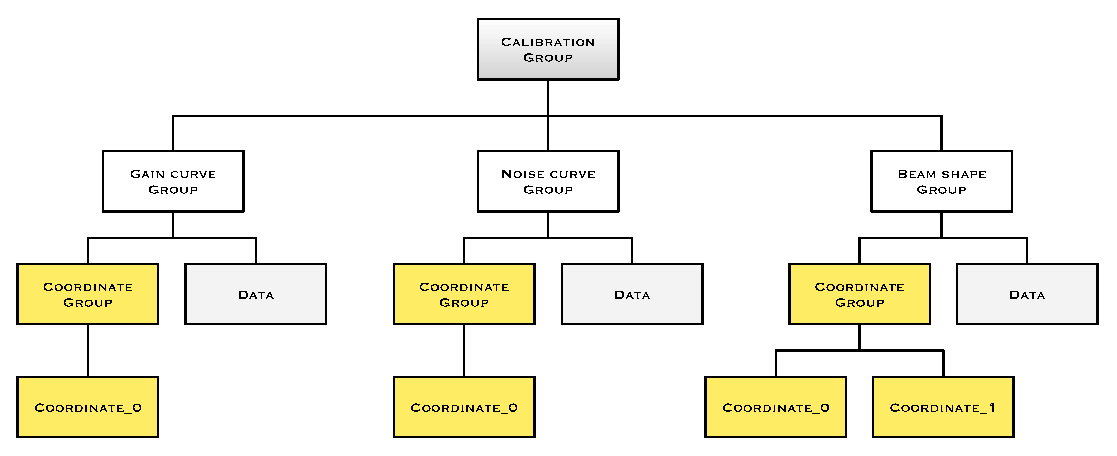
\includegraphics[width=\textwidth]{figures/TBB_CalibrationGroup.eps}
  \caption{Hierarchical structure of the station calibration
    group. Even though one could consider storing information such as
    the gain curve as simple attributes attached to the calibration
    group there are a number of arguments which speak against such
    course of action: a) An attribute can only be access via the
    object. b) For practical reasons, an attribute should be a small
    object, no more than 1000 bytes. c) The data of an attribute must
    be read or written in a single access, selection is not allowed.}
  \label{fig:station calibration group}
\end{figure}

\begin{table}[ht]
  \centering
  \begin{tabular}{|lllp{9cm}|}
    \hline
    \sc Field/Keyword & \sc H5Type & \sc Type & Description \\
    \hline \hline
    \verb|GROUPTYPE|        & Attr & \verb|string| & LOFAR group type,
    \texttt{StationCalibration}. \\
    \verb|GainCurve|       & Group &   & Sub-group storing physical coordinates
    and values of the complex electronic gain, $\mathbf G_{j,\rm gain} = G_{j}(\nu)$. \\
    \verb|NoiseCurve|      & Group &   & Sub-group storing physical coordinates
    and values of the complex electronic noise, $\mathbf G_{j,\rm noise} = G_{j}(\nu)$. \\
    \verb|BeamShape|       & Group &   & Sub-group storing physical coordinates
    and values of the complex element beam pattern as function of direction
    and frequency $\mathbf G_{\rm beam} = G (\vec \rho, \nu)$. \\
    \hline
  \end{tabular}
  \caption{Structure of the \textbf{Station calibration group};
    besides a number of top-level attributes, the group acts as a
    container for the actual calibration data, which are stored inside
    individual sub-groups.}
  \label{tab:station calibration group}
\end{table}

Each of the sub-groups for an individual calibration quantity, will consist of
a part describing the physical coordinates (e.g. a frequency axis) and an array
storing the actual calibration values:

\begin{list}{\textbf{--}}{}
\item \verb|GAIN_CURVE| : complex electronic gain, $\mathbf G_{j,\rm gain} = G_{j}(\nu)$,
  for receiving element $j$ as function of frequency (bandpass); this array
  will be multiplied (after interpolation, if required) to the output of the
  Fourier transform of the dipole voltage time-series.

 \begin{table}[ht]
    \centering
    \begin{tabular}{|lllp{6cm}|}
      \hline
      \sc Field/Keyword & \sc H5Type & \sc Type & Description \\
      \hline \hline
      \verb|GROUPTYPE|        & Attr. & \verb|string| & LOFAR group type,
      \verb|GainCurve| \\
      \verb|GAIN_CURVE_UNIT|  & Attr. & \verb|string|          &  \\
      \verb|NOF_COORDINATES|  & Attr. & \verb|int|             &
      Number of coordinate objects attached to this group. \\
      \verb|NOF_AXES|         & Attr. & \verb|int|             &
      Number of coordinate axes represented by the attached coordinate
      groups. \\
      \verb|COORDINATE_TYPES| & Attr. & \verb|array<string,1>| & Type
      of the attached coordinate objects. \\
      \hline 
      \verb|Coordinate_0|      & Group   &             & Coordinate
      object describing the frequency axis. \\
      \verb|GainCurveData|  & Dataset & \verb|array<complex,1>| &  \\
      \hline
    \end{tabular}
    \caption{Attributes, groups and dataset attached to the gain curve
      calibration group.}
    \label{tab:gain curve group}
  \end{table}
  {\small
%\begin{verbatim}
%.
%`-- Calibration                    Group
%    |-- GainCurve                  Group
%    |   |-- GROUPTYPE              Attr.     string              = 'GainCurve'
%    |   |-- GAIN_CURVE_UNIT        Attr.     string              = 
%    |   |-- NOF_COORDINATES        Attr.     int                 = 1
%    |   |-- NOF_AXES               Attr.     int                 = 1
%    |   |-- COORDINATE_TYPE        Attr.     array<string,1>     = ['Spectral']
%    |   |-- Coordinate_0            Group     
%    |   |   |-- GROUPTYPE          Attr.     string              = 'SpectralCoord'
%    |   |   |-- COORDINATE_TYPE    Attr.     string              = 'Spectral'
%    |   |   |-- STORAGE_TYPE       Attr.     string              = 'Linear'
%    |   |   |-- NOF_AXES           Attr.     int                 = 1
%    |   |   |-- AXIS_NAMES         Attr.     array<string,1>     = ['Frequency']
%    |   |   |-- AXIS_UNITS         Attr.     array<string,1>     = ['Hz']
%    |   |   |-- REFERENCE_VALUE    Attr.     array<double,1>     
%    |   |   |-- REFERENCE_PIXEL    Attr.     array<double,1>
%    |   |   |-- INCREMENT          Attr.     array<double,1>
%    |   |   `-- PC                 Attr.     array<double,1>      = [1.0]
%    |   `-- Data                   Dataset   array<complex,1>
%\end{verbatim}
  }
\item \verb|NOISE_CURVE| : complex electronic noise, $\mathbf G_{j,\rm noise} = G_{j}(\nu)$,
  for receiving element $j$ as function of frequency (bandpass); this array
  will be multiplied (after interpolation, if required) to the output of the
  Fourier transform of the dipole voltage time-series.
  \begin{table}[ht]
    \centering
    \begin{tabular}{|lllp{6cm}|}
      \hline
      \sc Field/Keyword & \sc H5Type & \sc Type & Description \\
      \hline \hline
      \verb|GROUPTYPE|        & Attr. & \verb|string| & LOFAR group type,
      \verb|NoiseCurve| \\
      \verb|NOISE_CURVE_UNIT|  & Attr. & \verb|string|          &  \\
      \verb|NOF_COORDINATES|  & Attr. & \verb|int|             &
      Number of coordinate objects attached to this group. \\
      \verb|NOF_AXES|         & Attr. & \verb|int|             &
      Number of coordinate axes represented by the attached coordinate
      groups. \\
      \verb|COORDINATE_TYPES| & Attr. & \verb|array<string,1>| & Type 
      of the attached coordinate objects. \\
      \hline 
      \verb|Coordinate_0|      & Group   &             & Coordinate
      object describing the frequency axis. \\
      \verb|NoiseCurveData|  & Dataset & \verb|array<complex,1>| &  \\
      \hline
    \end{tabular}
    \caption{Attributes, groups and dataset attached to the noise curve
      calibration group.}
    \label{tab:noise curve group}
  \end{table}
  {\small
%\begin{verbatim}
%.
%`-- Calibration                    Group
%    |-- NoiseCurve                 Group
%    |   |-- GROUPTYPE              Attr.     string              = 'NoiseCurve'
%    |   |-- NOISE_CURVE_UNIT       Attr.     string              = 
%    |   |-- NOF_COORDINATES        Attr.     int                 = 1
%    |   |-- NOF_AXES               Attr.     int                 = 1
%    |   |-- COORDINATE_TYPE        Attr.     array<string,1>     = ['Spectral']
%    |   |-- Coordinate_0            Group     
%    |   |   |-- GROUPTYPE          Attr.     string              = 'SpectralCoord'
%    |   |   |-- COORDINATE_TYPE    Attr.     string              = 'Spectral'
%    |   |   |-- STORAGE_TYPE       Attr.     string              = 'Linear'
%    |   |   |-- NOF_AXES           Attr.     int                 = 1
%    |   |   |-- AXIS_NAMES         Attr.     array<string,1>     = ['Frequency']
%    |   |   |-- AXIS_UNITS         Attr.     array<string,1>     = ['Hz']
%    |   |   |-- REFERENCE_VALUE    Attr.     array<double,1>     
%    |   |   |-- REFERENCE_PIXEL    Attr.     array<double,1>
%    |   |   |-- INCREMENT          Attr.     array<double,1>
%    |   |   `-- PC                 Attr.     array<double,1>      = [1.0]
%    |   `-- Data                   Dataset   array<complex,1>
%\end{verbatim}
  }
\item \verb|BEAM_SHAPE| holds the complex \textbf{element beam pattern} as
  function of direction and frequency $\mathbf G_{\rm beam} = G (\vec \rho, \nu)$.
  In order to correctly interpret the data -- and, if necessary, interpolate --
  the corresponding \textbf{beam directions} (\verb|BEAM_DIRECTIONS|) and
  \textbf{frequency values} (\verb|BEAM_FREQUENCIES|) are required.
  \begin{table}[ht]
    \centering
    \begin{tabular}{|lllp{6cm}|}
      \hline
      \sc Field/Keyword & \sc H5Type & \sc Type & Description \\
      \hline \hline
      \verb|GROUPTYPE|        & Attr. & \verb|string| & LOFAR group type,
      \verb|BeamShape| \\
      \verb|BEAM_SHAPE_UNIT|  & Attr. & \verb|string|          &  \\
      \verb|NOF_COORDINATES|  & Attr. & \verb|int|             &
      Number of coordinate objects attached to this group. \\
      \verb|NOF_AXES|         & Attr. & \verb|int|             &
      Number of coordinate axes represented by the attached coordinate
      groups. \\
      \verb|COORDINATE_TYPES| & Attr. & \verb|array<string,1>| & Type
      of the attached coordinate objects. \\
      \hline 
      \verb|COORDINATE_0|      & Group   &             & Coordinate
      object describing the directional axes. \\
      \verb|COORDINATE_1|      & Group   &             & Coordinate
      object describing the frequency axis. \\
     \verb|BEAM_SHAPE_DATA|  & Dataset & \verb|array<complex,3>| & The beam-shape data. \\
      \hline
    \end{tabular}
    \caption{Attributes, groups and dataset attached to the beam shape
      calibration group.}
    \label{tab:beam shape group}
  \end{table}
%{\small 
%\begin{verbatim}
%.
%`-- Calibration                    Group
%    |-- BeamShape                  Group
%    |   |-- GROUPTYPE              Attr.     string              = 'BeamShape'
%    |   |-- BEAM_SHAPE_UNIT        Attr.     string              = 
%    |   |-- NOF_COORDINATES        Attr.     int                 = 2
%    |   |-- NOF_AXES               Attr.     int                 = 3
%    |   |-- COORDINATE_TYPE        Attr.     array<string,1>     = ['Direction','Spectral']
%    |   |-- Coordinate_0           Group     
%    |   |   |-- GROUPTYPE          Attr.     string              = 'DirectionCoord'
%    |   |   |-- COORDINATE_TYPE    Attr.     string              = 'Direction'
%    |   |   |-- STORAGE_TYPE       Attr.     string              = 'Linear'
%    |   |   |-- NOF_AXES           Attr.     int                 = 2
%    |   |   |-- AXIS_NAMES         Attr.     array<string,1>     = ['Az','El']
%    |   |   |-- AXIS_UNITS         Attr.     array<string,1>     = ['deg','deg']
%    |   |   |-- REFERENCE_VALUE    Attr.     array<double,1>     
%    |   |   |-- REFERENCE_PIXEL    Attr.     array<double,1>     
%    |   |   |-- INCREMENT          Attr.     array<double,1>     
%    |   |   |-- PC                 Attr.     array<double,1>     = [1.0,0.0,0.0,1.0]
%    |   |   |-- EQUINOX            Attr.     string
%    |   |   |-- RADEC_SYS          Attr.     string
%    |   |   |-- PROJECTION         Attr.     string
%    |   |   |-- PROJECTION_PARAM   Attr.     array<double,1>
%    |   |   |-- LONGPOLE           Attr.     double
%    |   |   |-- LATPOLE            Attr.     double
%    |   |   |-- CONVERSION_SYSTEM  Attr.     string
%    |   |-- Coordinate_1           Group     
%    |   |   |-- GROUPTYPE          Attr.     string              = 'SpectralCoord'
%    |   |   |-- COORDINATE_TYPE    Attr.     string              = 'Spectral'
%    |   |   |-- STORAGE_TYPE       Attr.     string              = 'Linear'
%    |   |   |-- NOF_AXES           Attr.     int                 = 1
%    |   |   |-- AXIS_NAMES         Attr.     string     = ['Frequency']
%    |   |   |-- AXIS_UNITS         Attr.     string     = ['Hz']
%    |   |   |-- REFERENCE_VALUE    Attr.     array<double,1>     
%    |   |   |-- REFERENCE_PIXEL    Attr.     array<double,1>
%    |   |   |-- INCREMENT          Attr.     array<double,1>
%    |   |   `-- PC                 Attr.     array<double,1>      = [1.0]
%    |   `-- Data                   Dataset   array<complex,3>
%\end{verbatim}
%}
\end{list}


\subsection{Dipole Dataset}
\label{sec:dipole dataset}

The \textbf{Dipole Dataset} (Tab. \ref{tab:ANTENNA_TABLE}) collects data on
a per-dipole basis\footnote{Please keep in mind here, that we clearly
  distinguish between \textsl{antenna} and \textsl{dipole/feed}: using the
  feed-based approach as underlying the Measurement-Equation, an antenna can
  consist of multiple feeds (or dipoles).} -- starting from the identifiers
required for the unambiguous identification of an individual dipole within
the full LOFAR network to the actual sampled wave-form of the EM-field at the
position of each antenna feed.

N.B. In the discussion of subband data held in the payload of a frame, 'sample'
refers to the first subband as stored in the payload.

\begin{table}[htbp]
  \centering
  \begin{tabular}{|llp{7.5cm}|}
    \hline
    \sc Field/Keyword & \sc Type &  Description \\
    \hline \hline
    \verb|GROUPTYPE| & \texttt{string} & The type of this group, \textsl{DipoleDataset} \\
    \verb|STATION_ID| & \texttt{uint} & Data source station identifier \\
    \verb|RSP_ID| & \verb|uint| & Data source RSP board identifier \\
    \verb|RCU_ID| & \verb|uint| & Data source RCU board identifier \\
    \verb|SAMPLE_FREQUENCY_VALUE| & \verb|double| & Sample frequency in
    MHz of the RCU boards \\
    \verb|SAMPLE_FREQUENCY_UNIT| & \verb|string| & Physical units of the
    sample frequency. \\
    \verb|TIME| & \verb|uint| & Time instance in seconds of the first
    sample in the payload \\
    \verb|BAND_NUMBER| & \verb|uint| & Subband number of the first
    payload sample \\
    \verb|SLICE_NUMBER| & \verb|uint| & This number indicates the slice
    (i.e. a transformed block of 1024 samples) of the first payload sample \\
    \verb|SAMPLES_PER_FRAME| & \verb|uint| & Total number of samples
    in the payload of the original TBB--RSP frame structure \\
    \verb|NOF_SUBBANDS| & \verb|uint| & Number of subbands contained in a spectrum \\
    \verb|SUBBANDS| & \verb|uint| & List of all subbands selected; items are between
    and include 0 to 511 \\
    \verb|DATA_LENGTH| & \verb|uint| & The number of samples per dipole
    which actually stored into the data set; this might as well be different from
    the number of samples in a data frame \\
    \verb|NYQUIST_ZONE| & \verb|uint| & Nyquist zone in which the
    data are sampled \\
    \verb|ADC2VOLTAGE| & \verb|double| & Conversion factor from raw
    ADC sample values to voltages. \\
    \verb|CABLE_DELAY| & \verb|double| & Delay the length of the cable
    connected to the RCU adds to the signal path. \\
    \verb|CABLE_DELAY_UNIT| & \verb|string| & Physical unit associated
    with \verb|CABLE_DELAY|. \\
    \verb|FEED| & \verb|string| & Type of feed for this dipole \\
    \verb|ANTENNA_POSITION_VALUE| & \verb|array<double,1>| &
    [3] Antenna position w.r.t. the station center, $\vec x = (x_1,x_2,x_3)$ \\
    \verb|ANTENNA_POSITION_UNIT| & \verb|string| & Physical units
    of the antenna position \\
    \verb|ANTENNA_POSITION_FRAME| & \texttt{string} & Reference frame of the antenna position. \\
    \verb|ANTENNA_ORIENTATION_VALUE| & \verb|array<double,1>| & [3] Antenna orientation w.r.t. the reference frame within which the antenna positions are defined \\
    \verb|ANTENNA_ORIENTATION_UNIT| & \verb|string| & Physical
    units of the antenna orientation; depending on the convention used this might
    be \textsc{deg} or \textsc{m}. \\
    \verb|ANTENNA_ORIENTATION_FRAME| & \texttt{string} & Reference frame of the antenna orientation. \\
    \verb|TILE_BEAM_VALUE| & \verb|array<double,1>| &
    Numerical value of the tile beam direction \\
    \verb|TILE_BEAM_UNIT| & \verb|string| & Physical
    units of the tile beam orientation. \\
    \verb|TILE_BEAM_FRAME| & \texttt{string} & Reference frame of the tile beam.  \\
    \verb|TILE_BEAM_DIPOLES| & \verb|array<uint,1>| & Dipoles
    within the tiles, which were used for the beamforming.  \\
    \verb|TILE_COEF_UNIT| & \verb|string| & Physical units of the
    tile beam coefficients.\\
    \verb|TILE_BEAM_COEFS| & \verb|array<usint,1>| & Coefficients used
    in the analogue dipole beamformer for this beam.  \\
    \verb|TILE_DIPOLE_POSITION_VALUE| & \verb|array<double,3>| & Position of the dipoles within the tile. \\
    \verb|TILE_DIPOLE_POSITION_UNIT| & \verb|string| & Units of the tile dipole positions.\\
    \verb|TILE_DIPOLE_POSITION_FRAME| & \verb|string| & Reference frame of the dipole positions.\\
   \hline
  \end{tabular}
  \caption{Fields in the dipole dataset; each listed field
    corresponds to a column in the table, where the number of rows corresponds
    to the number of dipoles. The first set of values is adopted directly from
    the frame structure used for data transfer between TBB and RSP
    \cite{poiesz.2006}.}
  \label{tab:ANTENNA_TABLE}
\end{table}

\begin{comment}
  Add attribute to store values of the analoge beamformer for the HBA
  tiles.
\end{comment}


\begin{list}{\textbf{--}}{}
\item \verb|STATION_ID|, \verb|RSP_ID| and \verb|RCU_ID| are directly taken
  from the frame structure used in the communication between RSP and TBB 
  \cite{poiesz.2006}. The three identifiers -- in combination with
  \verb|ANTENNA_SET| in combination -- allow for an unambiguous
  identification of an individual dipole within the LOFAR network; 
  depending on the range of value of the individual numbers the unique ID
  may be constructed via e.g.
  \begin{equation}
    N_{\rm ID} = 10^4 \cdot N_{\rm Station} + 10^2 \cdot N_{\rm RSP} +
    N_{\rm RCU}
  \end{equation}
\item The combination of the two fields \verb|TIME| and \verb|SLICE_NUMBER|
  gives an absolute time reference for the first spectrum in the \verb|DATA|
  field. However, as a spectrum requires 1024 samples the timing is determined
  to within 5.12 microseconds at 200 MHz sampling frequency.
  The \verb|TIME| field gives a time offset in seconds from a certain
  start moment, where the LCU is completely free at chossing a time system,
  such as UNIX time\footnote{Referring to the UINX time, this field would hold
    the number of seconds since 1970}. For a constant sampling frequency
  (\verb|SAMPLE_FREQ|) the timing for the remaining spectra can be derived
  via \cite{poiesz.2006}
  \begin{equation}
    t[n] = t_{\rm TIME} + \left( t_{\rm SLICE_-NR} + n  \right) \cdot 1024
    \cdot 1/\nu_{\rm SAMPLE_-FREQ}
  \end{equation}
  where $n$ is the index for the n-th spectrum in the \verb|DATA| vector.
\item Each frame of data transferred between RSP and TBB has the same fixed
  length (\verb|SAMPLES_PER_FRAME|), but a frame may hold any number of samples
  that will fit in the payload area of the frame. As typically the
  number of samples requested from the TBB will be larger but the
  number of samples fitting into a single frame, the resulting dataset
  will accumulate the contents from multiple frames.
\item \verb|DATA| stores the raw ADC output for an individual signal path/dipole,
  consisting of \verb|DATA_LENGTH| samples for a single dump of TBB data; the
  length of this data vector will vary depending on the observation mode. \\
\item the \textbf{position} of the receiving element within the station:
  \begin{itemize} \parskip 0pt
  \item \verb|ANTENNA_POSITION_VALUE| -- numerical value of the antenna position
    coordinates
  \item \verb|ANTENNA_POSITION_UNIT| -- physical units associated with the numerical
    values for the antenna position
  \item \verb|ANTENNA_POSITION_FRAME| -- identifier for the reference frame within
    which the antenna position is provided
  \end{itemize}
\item the \textbf{orientation} of the receiving element w.r.t to the coordinate
  frame within which the position of the same element was provided:
  \begin{itemize}
  \item \verb|ANTENNA_ORIENTATION_VALUE|| -- numerical value of the parameters 
    describing the orientation of the antenna
  \item \verb|ANTENNA_ORIENTATION_UNIT| -- physical units associated with the
    numerical values for the antenna orientation
  \item \verb|ANTENNA_ORIENTATION_FRAME| -- identifier for the reference frame
    within which the antenna orientation is provided
  \end{itemize}
  An agreement on the format, in which this information is provided, still needs
  to be made, but it is foreseeable to describe the orientation (tilt) of an
  receiving element in one of the two ways:
  \begin{enumerate}
  \item Euler angles describing a rotation between the reference frame within 
    which the position of the antenna is given and the coordinate frame based on
    the antenna's orientation.
  \item Normal (unit length) vector indicating the orientation of the antenna
    from the location defined by the antenna position.
  \end{enumerate}
\end{list}

%%_______________________________________________________________________________
%%                                                                     Interfaces

\section{Interfaces}
\label{sec:interfaces}

\subsection{Interface requirements}
\label{sec:interface requirements}

\begin{itemize}
\item low-level generic interface to individual elements within the dataset 
  $\rightarrow$ provided by the DAL
\item high-level interface tranversing hierarchy boundaries $\rightarrow$ some
  of this initially not provided by the DAL itself, but later on integrated from
  external code base (such as e.g. CR-Tools)
  \begin{itemize}
  \item create/read/write attributes
  \item (sliced) reading of channel data
  \item creation of a new (empty) dataset
  \end{itemize}
\end{itemize}

\subsection{Relationship with other interfaces}

The functionality to write, access and inspect subband data will not come
from a single software components (as delivered by the USG), but requires
coverage by the following modules:
\begin{itemize}
\item Data Acces Library (DAL) -- to provide read/write access to the data,
  as physically located on storage media (single hard-drive, RAID array, GRID,
  etc.)
\end{itemize}
A detailed description of the expected interaction of above mentioned modules
is given in section \ref{sec:interfaces} (\textsl{Interfaces}).

\subsection{Relation to existing workpackages}

\paragraph{Data Access Library (DAL)}

While in most usage scenarios all the valid data from a LOFAR station will
be read in to be processed together, their might be the need to select data
from antenna across the borders of a LOFAR station: this will require the
ability to access data based on the geographical locations, such as e.g.
\begin{list}{\textbf{--}}{} \parskip 0pt
\item all antennas within a N Kilometer radius of the shower core
\item all antennas within a sector of M degrees opening angle towards a given
  direction w.r.t. the shower core
\item all antennas located in a ring of $N_1 < R < N_2$ around the position
  of the shower core
\end{list}

%%_______________________________________________________________________________
%%                                                          Section: Requirements

\section{Requirements}
\label{sec:requirements}

\subsection{Metadata}
\label{sec:metadata}

Metadata is the auxiliary data stored along with the subband data needed to
provide all the necessary information for automated processing of the data.
This data can either be stored directly in the data set or it can be stored
in an external database. In the latter case the data set must contain a
pointer to the correct entry in that database (e.g. the antenna-id is needed
to get the antenna position).

\begin{itemize} \parskip 0pt
\item DAQ mode, including Samplerate, Filters, etc.
\item Timing information:
  \begin{itemize}
  \item Trigger time relative to recorded data segement
  \item Timing of the data streams relative to the trigger
  \item Timing of the data streams relative to each other with sub-sample
    accuracy; This can be implicit, e.g. all data streams of a station start
    at the same time. Fields that can be in stored in an external database.
  \end{itemize}
\item List of RFI sources identified by the station calibration, including
  \textbf{direction}, \textbf{center frequency} and \textbf{peak strength}.
  \begin{list}{$\rightarrow$}{}
  \item What does this actually mean: the properties of the single channel
    containing the highest signal level or the parameters obtained from fitting
    e.g. a Gaussian to a segment of the spectrum?
  \end{list}
\item dispersion measure of the ionosphere (at this point in time and space)
\item health information about the antennas
\end{itemize}

\subsubsection{System monitoring and system health.}

Information on the status of the various (hardware) components at a LOFAR station
will be stored inside the PVSS database; a description of the datapoint-types and
datapoints can be found in the \verb|MAC/Deployment/data/PVSS| branch of the
LOFAR code repository (see Tab. \ref{tab:PVSS} for an excerpt).

\begin{table}[htb]
  \centering
  \begin{tabular}{|lll|}
    \hline
    \sc Database entry & \sc Field & \sc Format \\
    \hline \hline
    CalCtlr & connected    & bool \\
            & obsname      & string \\
            & antennaArray & string \\
            & filter       & string \\
            & nyquistzone  & int \\
            & rcus         & string \\
    \hline
    ObservationControl & claimPeriod & int \\
    & preparePeriod   & int \\
    & startTime       & string \\
    & stopTime        & string \\
    & subbandList     & string \\
    & beamletList     & string \\
    & bandFilter      & string \\
    & nyquistzone     & int \\
    & antenneArray    & string \\
    & receiverList    & string \\
    & sampleClock     & int \\
    & measurementSet  & string \\
    & stationList     & string \\
    & inputNodeList   & string \\
    & BGLNodeList     & string \\
    & storageNodeList & string \\
    \hline
  \end{tabular}
  \caption{Excerpt from the list of entries into the PVSS database. The
    definitions of the datapointtypes and datapoints can be found in the
    \texttt{MAC/Development/data/PVSS} branch of the LOFAR code repository.}
  \label{tab:PVSS}
\end{table}

In order to later store certain system health information along with the other
data, parameters need to be subscribed to at the definition of the observation.

\subsection{Visualization}

Past experience with the software for the LOPES experiment has shown, that is
is crucial to provide the user with a variety of way to graphically inspect
the data. This not only includes visualization of the time-series/FFT/etc.
data themselves, but also displaying the various data with the wider context
of the experimental setup (e.g. geographical distribution of the antennas
w.r.t. to the particle detector setup)

\begin{itemize}
\item Display of the standard data products (also see documentation of the
  \lopestools\ \verb|DataReader|): ADC, Voltage, FFT, Calibrated FFT,
  RFI-filtered FFT, Cross-Corr. Spectra, Visibilities
\item Display of the (intermediate) data products generated from the input
  data, e.g. dynamic spectra, multi-dimensional skymaps
\item Flags and weights associated with the data, e.g. filter curves, antenna
  gain curves, etc.
\item Station layout, i.e. positions of the (selected/excluded) antennas
\item antenna power level distribution over the area of the station/array
  (this is very similar to the type of event display as known from particle
  physics experiments)
\item mapping of the (local) RFI via an (Azimuth,Frequency) plot centered on
  the position of a certain station
\item geographical locations of identified RFI sources; such a plot should
  also indicate the  frequency band of the RFI (via label or bar etc.)
\item geographical distribution/location of antennas which generated a trigger
  signal, failed, etc.
  \begin{itemize}
  \item[$\rightarrow$] VR setting, combining geographical information (e.g.
    map of the Netherlands) with the location of localized CR-/TS-events
  \item[$\Rightarrow$] in a cave-like setup we actually can perform a
  fly-through, which would be ideal for outreach purposes!
  \end{itemize}
\item cummulative geographical distribution of detected CR events
\item total power per LOFAR station (geographically distributed)
\item overlay of CR data with information from other sensors (e.g. weather
  radar images, temperatures, etc.)
\end{itemize}
A number of the before-mentioned displayes should be interactive, in the sense
that the user should be able to perform data selection from the graphical
display (e.g. by drawing a circle around the core of the CR air shower,
thereby selecting the antennas included in the data analysis step).

%% ==============================================================================
%%
%%  Appendix
%%
%% ==============================================================================

\clearpage
\appendix

%%_______________________________________________________________________________
%%                                              Section: Anticipated Data volumes

\section{Anticipated Data volumes}
\label{sec:data volumes}

The data format needs to be able to handle data volumes as different as a
CR event with 1ms worth of data from a few antennas only to a full dump of 1
second worth of data from all LOFAR antennas in a consistent and efficient way.
The user may choose to dump as little as 1 subband or dump 487 subbands, which
is the maximum number of subbands.
Therefore, he figures below have been calculated per subband.

\begin{description}
\item[UHEP:]\ \\[2mm]
  \sumline{Time series data from the formed beam\\
    $ \hbox{2 pol} \times
    2^{27} \hbox{ samples} \times 2 \times
    8 \hbox{ Bytes/sample} \times 1/487 \hbox{ p. subband}$:}{\\8.8\,MB/event}
  \sumline{Raw time series data from individual dipoles\\
    $  77 \hbox{ stations} \times
    48 \hbox{ antennae} \times
    2 \hbox{ pol} \times
    2^{17} \hbox{ samples} \times 2 \times
    2 \hbox{ Bytes/sample} \times 1/487 \hbox{ p. subband}$:}{\\\underline{8.0\,GB/event}}
  \sumline{Total:}{17\,MB/event}
\item[VHECR:]\ \\[2mm]
  \sumline{Raw time series data from individual dipoles\\
   % $ 32 \hbox{ core stations} \times
    $48 \hbox{ antennae} \times
    2 \hbox { pol} \times
    2^{17} \hbox{ samples} \times 2 \times
    2 \hbox{ Bytes/sample} \times 1/487 \hbox{ p. subband}$:}{\\0.10\,MB/event}
\item[HECR:]\ \\[2mm]
  \sumline{Similar, but now only one station is involved\\
    $ 48 \hbox{ antennae} \times
    2 \hbox { pol} \times
    2^{17} \hbox{ samples} \times 2 \times
    2 \hbox{ Bytes/sample} \times 1/487 \hbox{ p. subband}$:}{\\0.10\,MB/event}
\item[TS-mode] \ \\[2mm]
  \sumline{Similar to VHECR but full raw data from TBB\\
    $ 77 \hbox{ stations} \times
    48 \hbox{ antennae} \times
    2 \hbox{ pol} \times
    2 \cdot 10^{8} \hbox{ samples} \times 2 \times
    2 \hbox{ Bytes/sample} \times 1/487 \hbox{ p. subband}$:}{\\12.0\,GB/event}
\end{description}

The event rate is uncertain, and for VHECR is estimated at one triggered event per station
per 10 minutes. With 32 stations active this would amount to 190 MB per subband per day of observing time.

%%_______________________________________________________________________________
%%                                                 Section: LOFAR common glossary

\section*{\glossaryname}
\label{sec:glossary}
\addcontentsline{toc}{section}{\glossaryname}

\input lofar_common_glossary

%%_______________________________________________________________________________
%% Bibliography

\bibliographystyle{plain}
\bibliography{references}

\end{document}
